\documentclass[a4paper, 11pt]{article}   %% Подешавање димензије странице, A4

\usepackage[utf8]{inputenc}         %% Encode as UTF-8
\usepackage[T2A]{fontenc}            %% Latin font

\usepackage[margin=1in]{geometry}	%% Margin settings
\usepackage[serbian]{babel}		    %% Srpski jezik
\usepackage{icomma}                 %% Srbizovanje decimalnog zareza
\usepackage{amsmath, amssymb}		%% Paketi za matematiku
\usepackage{enumitem}
\usepackage{tcolorbox}

\usepackage{graphicx}					%% Коришћење слика
\usepackage{subcaption}					%% Једна поред друге слике
\usepackage{wrapfig}                    %% Слика поред текста
\usepackage{booktabs}					%% Лепше, прегледније хоризонталне линије у табелама
\usepackage{float}						%% Омогућава опцију [H] за фиксирање позиције слике/табеле
\usepackage{pgfplots}					%% Цртање графика директно из \LaTeX-а на основу нумеричких података
\pgfplotsset{compat=1.18}				%% Верзија компатибилности pgfplots пакета

\usepackage{xcolor}					    %% Боје, потребне пакету listings за осенчавање синтаксе
\usepackage{listings}					%% Исечци изворног кода са осенчавањем синтаксе

\lstset{
    basicstyle=\ttfamily\small,
    keywordstyle=\color{blue!70!black}\bfseries,
    commentstyle=\color{gray},
    stringstyle=\color{green!50!black},
    numbers=left,
    numberstyle=\tiny,
    breaklines=true,
    frame=single,
    showstringspaces=false
}
\usepackage{algorithm}					%% Плутајуће окружење за алгоритме (наслов, ознака, листа алгоритама)
\usepackage{algpseudocode}				%% Псеудокод: \State, \For, \If итд.

\renewcommand{\lstlistingname}{Isečak koda}	    %% Преводи наслов "Listing" -> "Исечак кода"
\floatname{algorithm}{Algoritam}				%% Преводи наслов "Algorithm" -> "Алгоритам"

\usepackage[Symbolsmallscale]{upgreek}  %% Пакет за усправна грчка слова
\usepackage{indentfirst}				%% Увлачење првог пасуса

% \usepackage[backend=biber, style=numeric, sorting=none]{biblatex} %% Модеран начин вођења библиографије
% \addbibresource{literatura.bib}         %% Фајл са референцама (BibTeX/biblatex формат), треба га направити одвојено

\usepackage{hyperref}					%% Пакет hyperref омогућава клика-билне линкове -- како унутрашње
										%% референце (садржај, \ref, \cite), тако и спољашње URL адресе
										%% преко команде \href{URL}{текст који се приказује}, нпр:
										%% \href{https://www.overleaf.com}{Overleaf}. Пакет се увек учитава
										%% последњи у преамбули, јер редефинише многе команде других пакета.
\hypersetup{
    colorlinks=true,
    linkcolor=black,
    citecolor=black,
    urlcolor=blue
}

%%%%% Наменске команде које дефинишу често коришћене ствари у
%%%%% одговарајућем стилу. Команде треба користити

%% Ознаке јединице се куцају усправним словима, са МАЛИМ размаком 
%% испред ознаке јединице:
\newcommand{\unit}[1]{\,\mathrm{#1}}	%% Ознака јединице, \unit{V}

%% Математичке константе се куцају усправним словима (j, e, pi)
\newcommand{\jj}[1]{\mathrm{j}}	    	%% Комплексна јединица, \jj 
\newcommand{\ee}[1]{\mathrm{e}}			%% Ојлерова константа, \ee

%% Команде можете дефинисати и сами 



%%% Део документа до овог места назива се ПРЕАМБУЛА, и садржи све дефиниције пакета, 
%%% команди, околина итд. Од линије \begin{document} почиње опис самог документа. 


%%%% DOCUMENT START

\begin{document}

\thispagestyle{empty} % Bez numeracije

\begin{center}\Large
    \textsc{Univerzitet u Beogradu \\ Elektrotehnički fakultet} \\
    \vfill
    
\includegraphics[scale=1]{Resources/linijski.eps}
\end{center}

\vfill


\begin{center}
    % LARGE команда значи да се текст у наставку треба сложити ВЕЛИКИМ фонтом
    \huge Dosadašnji učinak u izradi diplomskog rada\\
    \textit{ \Large Implementacija digitalno upravljanog MPPT-a na \\
    topologiji Boost konvertora \\
    (WORKING TITLE - PRONE TO CHANGE)}
    % Или Мастер рад, или извештај са праксе
    % или друга слична обавеза. 
\end{center}

\vfill
\vfill % Последњи \vfill на страници, све испод ће бити погурано на дно странице

% Име кандидата и ментора. Minipage се користи када желимо да хоризонтално поређамо садржај. Могуће га је 
% користити и у другим околностима, али овде се показује нарочито користан. У суштини представља LaTeX 
% поддокумент (са неким ограничењима), назначене ширине
\noindent
\begin{minipage}{0.5\textwidth}
    \large
    Kandidat: \\ 
    Nikola Ristanović, \\ br. indeksa 2022/0469
\end{minipage}
%
\begin{minipage}{0.5\textwidth}
    \large
    \begin{flushright} % Околина поравнава текст уз десну ивицу. 
        Mentor: \\
        Dr Predrag Pejović \\ 
        redovni profesor
    \end{flushright}
\end{minipage}

\vspace{20mm}  % Вертикални размак, ширине тачно 20mm

\begin{center}
    \large
    Beograd, \today
\end{center}

\newpage % Форсирање нове странице

\,

\vfill



\begin{abstract}
    Izrada ovog diplomskig rada nažalost i dalje traje, većim delom zbog izražene neodlučnosti u domenu odabira komponenata i gabarita koje bi trebalo postići,\\
     a da i dalje postignu dovoljno dobre rezultate za potrebu testiranja i kvaliteta diplomskog rada.
    
    \vspace{1cm}
    
    With that in mind - Trenutno stanje je sledece:
    \begin{itemize}
        \item Sve komponente prikazane na semi \ref{schematic} su zalemljene na pertinaksu \ref{fig}
        \item Prilikom rada DC-DC konvertora dobijaju se ocekivani oblici napona i struja \ref{plot:Converter_Cycle_V&I}
        \item HAL za mikrokontroler je uredjen i testiran
        \item Kod za mikrokontroler jos nije odkucan, o tome ce biti reci posle
        \item Pristupi koji dolaze do mikrokontrolera se ponasaju kao sto je zamisljeno
    \end{itemize}
    
    \vspace{1cm}
    
    Na kraju ovog fajla ostavljam pitanja/hipoteze na koje nisam nasao odgovor i jako bi mi znacio input\\
    Takodje sam vise nego otvoren za sve savete i kritike, \textit{\textbf{cak i ako one ne bi bile realne za implementaciju u ovom trenutku, bilo zbog vremena, novca,
    ili tehnicke slozenosti - buduci da je ovo prilika za razmisljanje i ucenje}}, sto je i najveci razlog sto ovaj rad jos nije finaliziran.  
    
    
    \vspace{1cm}
    
    Takodje ceo dosadasnji razvoj ovog rada je u \href{https://github.com/NikolaRistanovic/Diplomski_rad}{Github repozitorijumu},
     gde postoje konkretna merenja u \textit{\textbf{.npy}} fajlova

    

    
\end{abstract}

\vfill

\,

\newpage

% Садржај  сложен према дефинисаним секцијама у 
% тексту, помоћу команди \section, \subsection, ...
% Уколико желите да се неко пот/поглавље не нађе у 
% садржају, користите команде које се завршавају на *
% нпр, \section*, \subsection*, ...
\tableofcontents 

\newpage 


\section{Hardver}
\label{sec:Hardver}

\subsection{Implementacija Boost konvertora}

Odabir vrednosti komponenti za konvertor se zasnivao na umanjenju ripple-a i dobrim delom je zasnovan na 
kupljenim boost konvertorima baziranim na LM2596. 

Idejni gabariti su bili:
\begin{itemize}
    \item Vin: 35V
    \item Vout: 50V
    \item Iin: 2A
    \item fs: 100kHz
    \item Vout\textsubscript{ac}: Minimalno - Realnu referencu nemam
\end{itemize}

\begin{figure}[h]
    \centering
    \includegraphics[width=\textwidth]{Resources/PDFs/PowerA.pdf}
    \caption{Elektricna sema boost konvertora}
    \label{schematic:Boost}
\end{figure}

Vrednost otpornosti kalema L1 \ref{img:Inductor} sa seme je procena, buduci da nisam imao nacin da je izmerim. Kalem nazivno ima maksimalnu struju od 3A,
stvarna struja zasicenja moze da se izmeri ako bi doprinela radu.


\noindent
Ulazni i izlazni filter kondenzaori imaju napon proboja od 63V.


\noindent
\href{https://www.st.com/en/diodes-and-rectifiers/stps2h100.html}{Dioda D1} ima maksimalni inverzni napon od 100V, i maksimalnu struju od 2A
Strujni senzori imaju maksimalnu dozvoljenu struju od 5A, o strujnim senzorima ce biti vise reci u \ref{sec:Akvizicija}

\vspace{1cm}

Jedno od velikih pitanja je sledece:"Kolika je procenjena vrednost paraztne induktivnosti \textbf{Metal-film} otpornika",
 buduci da od referenci koje sam upseo da nadjem - zbog tehnologije izrade trebalo bi da bude reda velicina nH. 
Na osnovu grafika struje kalema(napona na R1) i napona kalema L1, dolazi se do procenjenje vrednosti od ~500nH.
Koji je potencijalni metod merenja struje u ovom slucaju, a kojim nebi dolazili do znacajnog preslikavanja napona na kalemu L1?


\newpage


\section{Merenja}

\textit{Metode koje su koriscene za merenje ce biti obradjene u \hyperref[app:A]{Appendix A}}

\begin{figure}[h]
    \centering
    \includegraphics[width=\textwidth]{Resources/Plots/ForSafeKeeping.png}
    \caption{Vremenski oblici struja i napona u konvertoru}
    \label{plot:Converter_Cycle_V&I}
\end{figure}


\section{Appendix A}
\label{app:A}

\pagebreak
\section{Appendix B}
\label{app:B}
\begin{figure}[th]
    \centering
    \begin{minipage}{0.48\textwidth}
        \centering
        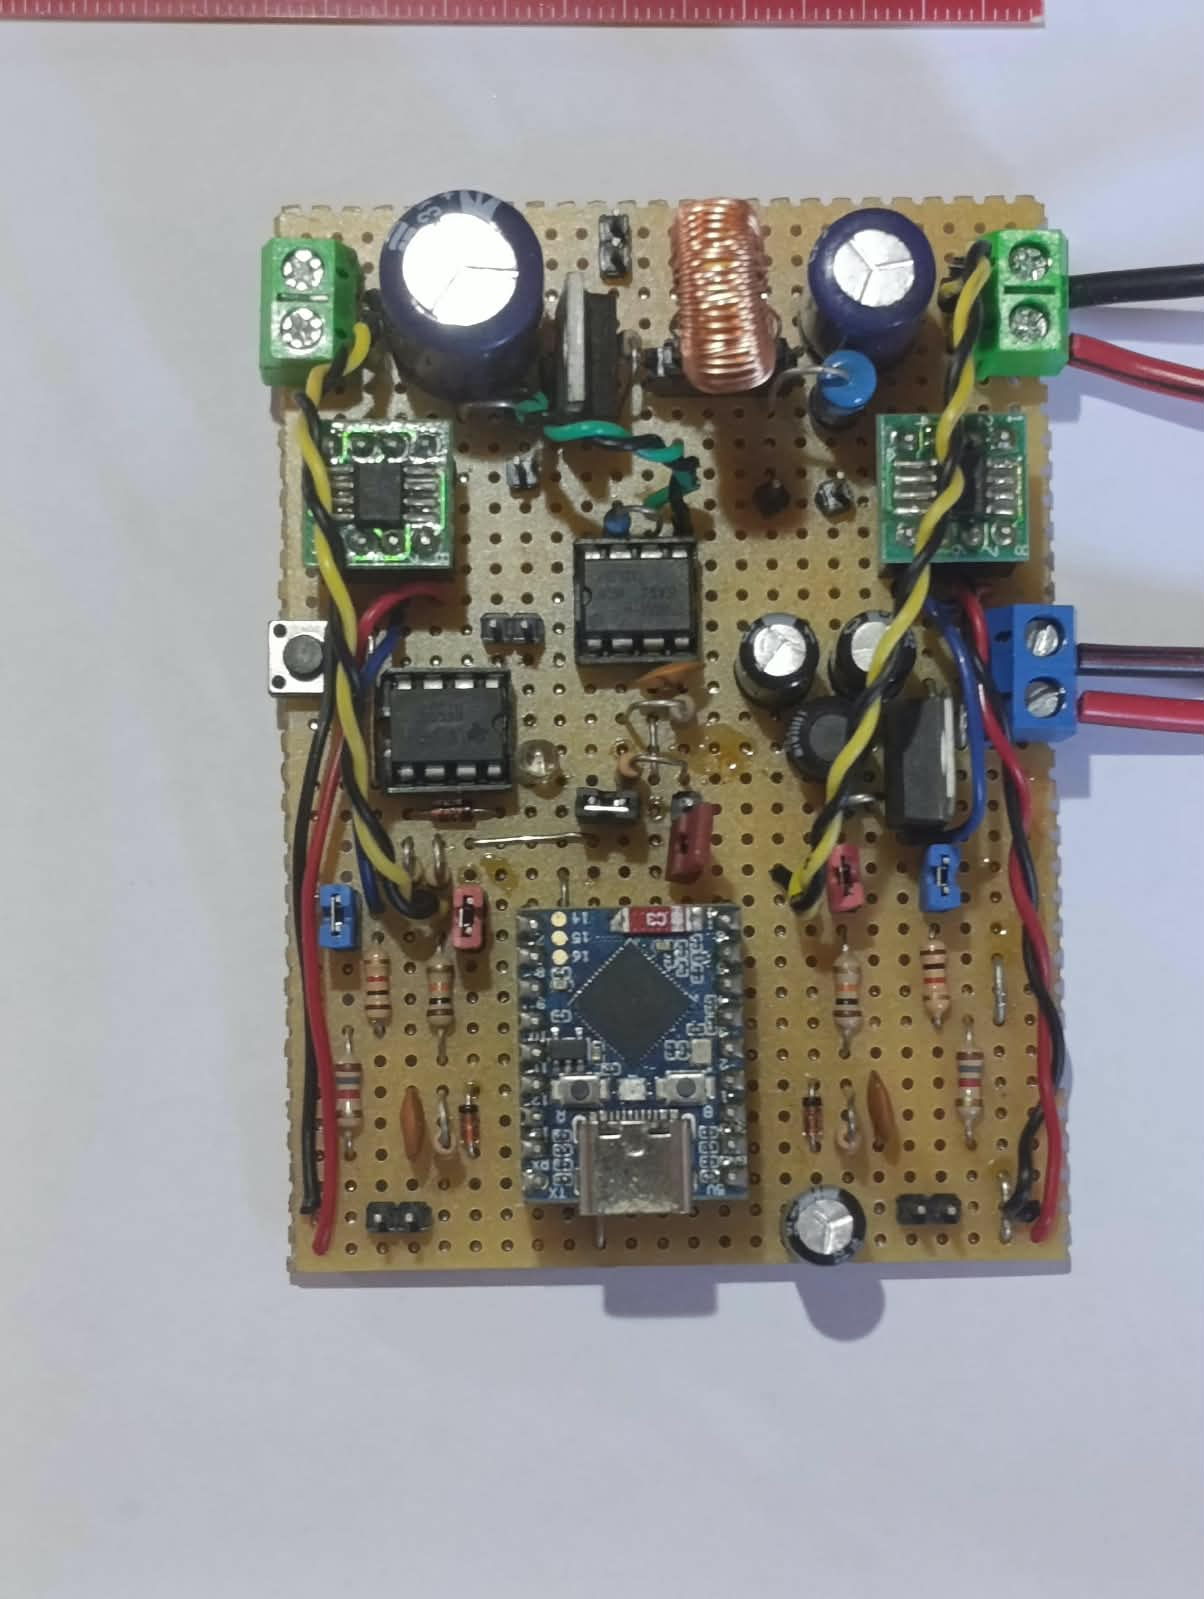
\includegraphics[width=\linewidth]{Resources/Images/Board_Front.jpeg}
        \caption{Prednja strana ploce}
        \label{img:Board_Front}
    \end{minipage}
    \hfill
    \begin{minipage}{0.48\textwidth}
        \centering
        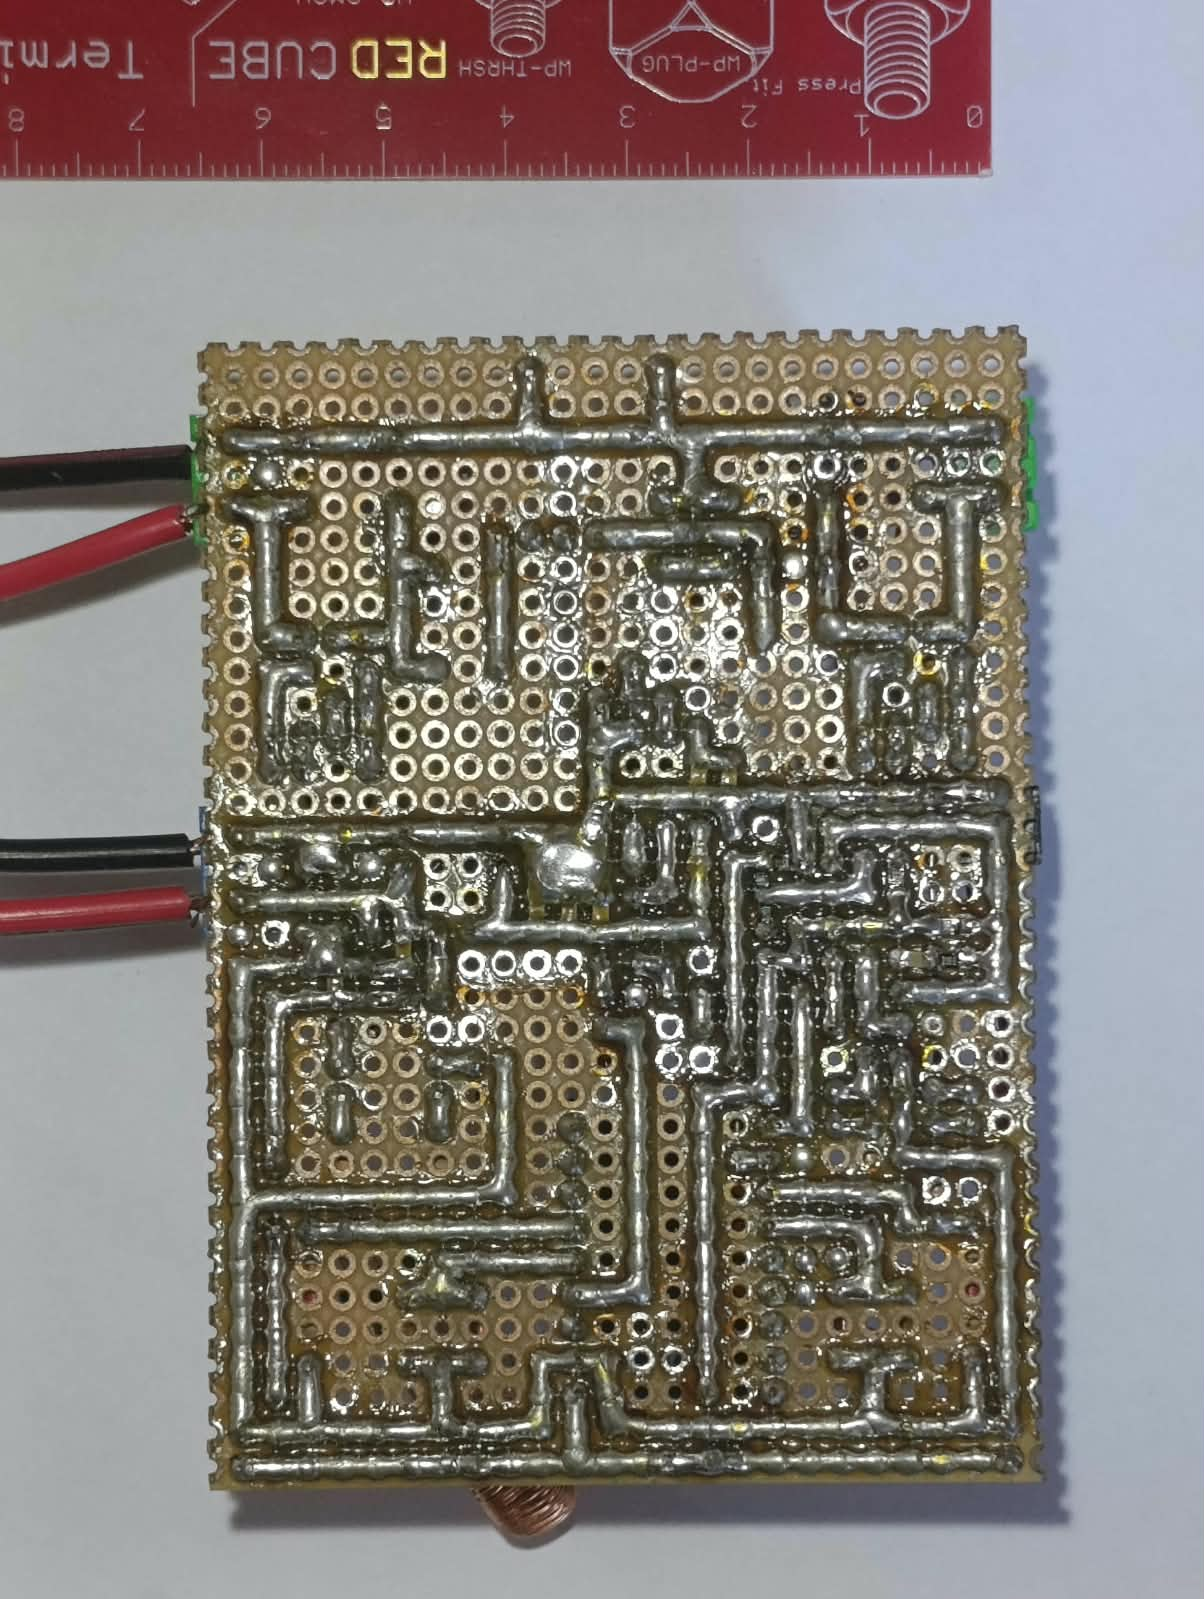
\includegraphics[width=\linewidth]{Resources/Images/Board_back.jpeg}
        \caption{Zadnja strana ploce}
        \label{plot:Board_back}
    \end{minipage}
    

    
\end{figure}

\pagebreak

% \begin{figure}[h]
    \section{Appendix C}
    \label{app:C}
        \begin{center}
            \includegraphics[width=\linewidth]{Resources/PDFs/PowerA.pdf}
        \end{center}
        \begin{center}
            \includegraphics[width=0.45\linewidth]{Resources/PDFs/Power.pdf}
            \includegraphics[width=0.45\linewidth]{Resources/PDFs/Driver.pdf}
        \end{center}
        \begin{center}
            \includegraphics[width=0.4\linewidth]{Resources/PDFs/Clipping.pdf}
            \includegraphics[width=0.4\linewidth]{Resources/PDFs/MCU.pdf}
        \end{center}
        \begin{center}
            \includegraphics[width=0.6\linewidth]{Resources/PDFs/Supply.pdf}
        \end{center}
% \end{figure}


\end{document}